\section{Model2DRigid  Class Reference}
\label{class_Model2DRigid}\index{Model2DRigid@{Model2DRigid}}
A holonomic rigid robot in a 2D world. 


{\tt \#include $<$model2d.h$>$}

Inheritance diagram for Model2DRigid::\begin{figure}[H]
\begin{center}
\leavevmode
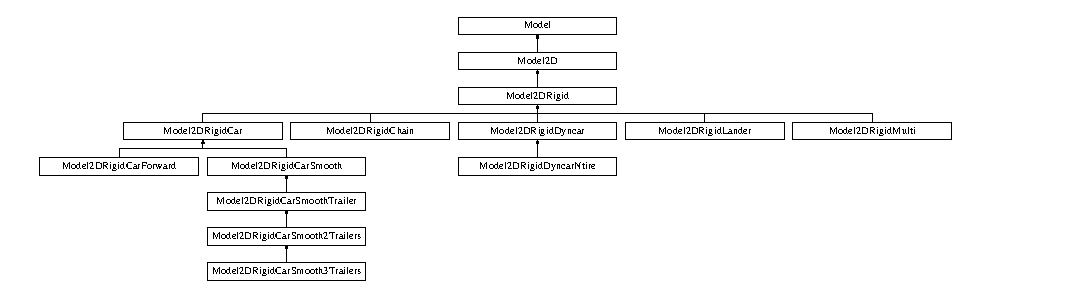
\includegraphics[height=3.5387cm]{class_Model2DRigid}
\end{center}
\end{figure}
\subsection*{Public Methods}
\begin{CompactItemize}
\item 
{\bf Model2DRigid} (string path)
\item 
virtual {\bf $\sim$Model2DRigid} ()
\item 
virtual {\bf MSLVector} {\bf Integrate} (const {\bf MSLVector} \&x, const {\bf MSLVector} \&u, const double \&h)
\begin{CompactList}\small\item\em Perform integration from state x, using input u, over time step h.\item\end{CompactList}\item 
virtual {\bf MSLVector} {\bf State\-Transition\-Equation} (const {\bf MSLVector} \&x, const {\bf MSLVector} \&u)
\begin{CompactList}\small\item\em The state transition equation, or equations of motion, xdot=f(x,u).\item\end{CompactList}\item 
{\bf MSLVector} {\bf Linear\-Interpolate} (const {\bf MSLVector} \&x1, const {\bf MSLVector} \&x2, const double \&a)
\begin{CompactList}\small\item\em Linearly interpolate two state while respecting topology.\item\end{CompactList}\item 
virtual double {\bf Metric} (const {\bf MSLVector} \&x1, const {\bf MSLVector} \&x2)
\begin{CompactList}\small\item\em A distance metric, which is Euclidean in the base class.\item\end{CompactList}\item 
virtual {\bf MSLVector} {\bf State\-To\-Configuration} (const {\bf MSLVector} \&x)
\begin{CompactList}\small\item\em A method that converts a {\bf Model} {\rm (p.\,\pageref{class_Model})} state in to a {\bf Geom} {\rm (p.\,\pageref{class_Geom})} configuration.\item\end{CompactList}\end{CompactItemize}


\subsection{Detailed Description}
A holonomic rigid robot in a 2D world.



\subsection{Constructor \& Destructor Documentation}
\index{Model2DRigid@{Model2DRigid}!Model2DRigid@{Model2DRigid}}
\index{Model2DRigid@{Model2DRigid}!Model2DRigid@{Model2DRigid}}
\subsubsection{\setlength{\rightskip}{0pt plus 5cm}Model2DRigid::Model2DRigid (string {\em path})}\label{class_Model2DRigid_a0}


\index{Model2DRigid@{Model2DRigid}!~Model2DRigid@{$\sim$Model2DRigid}}
\index{~Model2DRigid@{$\sim$Model2DRigid}!Model2DRigid@{Model2DRigid}}
\subsubsection{\setlength{\rightskip}{0pt plus 5cm}Model2DRigid::$\sim$Model2DRigid ()\hspace{0.3cm}{\tt  [inline, virtual]}}\label{class_Model2DRigid_a1}




\subsection{Member Function Documentation}
\index{Model2DRigid@{Model2DRigid}!Integrate@{Integrate}}
\index{Integrate@{Integrate}!Model2DRigid@{Model2DRigid}}
\subsubsection{\setlength{\rightskip}{0pt plus 5cm}virtual {\bf MSLVector} Model2DRigid::Integrate (const {\bf MSLVector} \& {\em x}, const {\bf MSLVector} \& {\em u}, const double \& {\em h})\hspace{0.3cm}{\tt  [virtual]}}\label{class_Model2DRigid_a2}


Perform integration from state x, using input u, over time step h.



Reimplemented from {\bf Model} {\rm (p.\,\pageref{class_Model_a5})}.

Reimplemented in {\bf Model2DRigid\-Car\-Smooth} {\rm (p.\,\pageref{class_Model2DRigidCarSmooth_a3})}, {\bf Model2DRigid\-Dyncar} {\rm (p.\,\pageref{class_Model2DRigidDyncar_a2})}, and {\bf Model2DRigid\-Lander} {\rm (p.\,\pageref{class_Model2DRigidLander_a2})}.\index{Model2DRigid@{Model2DRigid}!LinearInterpolate@{LinearInterpolate}}
\index{LinearInterpolate@{LinearInterpolate}!Model2DRigid@{Model2DRigid}}
\subsubsection{\setlength{\rightskip}{0pt plus 5cm}{\bf MSLVector} Model2DRigid::Linear\-Interpolate (const {\bf MSLVector} \& {\em x1}, const {\bf MSLVector} \& {\em x2}, const double \& {\em a})\hspace{0.3cm}{\tt  [virtual]}}\label{class_Model2DRigid_a4}


Linearly interpolate two state while respecting topology.

If a=0, then x1 is returned; if a=1, then x2 is returned. All intermediate values of \$a $\backslash$in [0,1]\$ yield intermediate states. This method is defined by {\bf Model} {\rm (p.\,\pageref{class_Model})}. 

Reimplemented from {\bf Model} {\rm (p.\,\pageref{class_Model_a6})}.

Reimplemented in {\bf Model2DRigid\-Dyncar} {\rm (p.\,\pageref{class_Model2DRigidDyncar_a6})}, {\bf Model2DRigid\-Multi} {\rm (p.\,\pageref{class_Model2DRigidMulti_a4})}, and {\bf Model2DRigid\-Chain} {\rm (p.\,\pageref{class_Model2DRigidChain_a4})}.\index{Model2DRigid@{Model2DRigid}!Metric@{Metric}}
\index{Metric@{Metric}!Model2DRigid@{Model2DRigid}}
\subsubsection{\setlength{\rightskip}{0pt plus 5cm}virtual double Model2DRigid::Metric (const {\bf MSLVector} \& {\em x1}, const {\bf MSLVector} \& {\em x2})\hspace{0.3cm}{\tt  [virtual]}}\label{class_Model2DRigid_a5}


A distance metric, which is Euclidean in the base class.



Reimplemented from {\bf Model} {\rm (p.\,\pageref{class_Model_a9})}.

Reimplemented in {\bf Model2DRigid\-Car\-Smooth} {\rm (p.\,\pageref{class_Model2DRigidCarSmooth_a4})}, {\bf Model2DRigid\-Car\-Smooth\-Trailer} {\rm (p.\,\pageref{class_Model2DRigidCarSmoothTrailer_a3})}, {\bf Model2DRigid\-Car\-Smooth2Trailers} {\rm (p.\,\pageref{class_Model2DRigidCarSmooth2Trailers_a3})}, {\bf Model2DRigid\-Car\-Smooth3Trailers} {\rm (p.\,\pageref{class_Model2DRigidCarSmooth3Trailers_a3})}, {\bf Model2DRigid\-Dyncar} {\rm (p.\,\pageref{class_Model2DRigidDyncar_a5})}, {\bf Model2DRigid\-Lander} {\rm (p.\,\pageref{class_Model2DRigidLander_a5})}, {\bf Model2DRigid\-Multi} {\rm (p.\,\pageref{class_Model2DRigidMulti_a2})}, and {\bf Model2DRigid\-Chain} {\rm (p.\,\pageref{class_Model2DRigidChain_a5})}.\index{Model2DRigid@{Model2DRigid}!StateToConfiguration@{StateToConfiguration}}
\index{StateToConfiguration@{StateToConfiguration}!Model2DRigid@{Model2DRigid}}
\subsubsection{\setlength{\rightskip}{0pt plus 5cm}virtual {\bf MSLVector} Model2DRigid::State\-To\-Configuration (const {\bf MSLVector} \& {\em x})\hspace{0.3cm}{\tt  [virtual]}}\label{class_Model2DRigid_a6}


A method that converts a {\bf Model} {\rm (p.\,\pageref{class_Model})} state in to a {\bf Geom} {\rm (p.\,\pageref{class_Geom})} configuration.



Reimplemented from {\bf Model2D} {\rm (p.\,\pageref{class_Model2D_a2})}.

Reimplemented in {\bf Model2DRigid\-Car\-Smooth} {\rm (p.\,\pageref{class_Model2DRigidCarSmooth_a5})}, {\bf Model2DRigid\-Car\-Smooth\-Trailer} {\rm (p.\,\pageref{class_Model2DRigidCarSmoothTrailer_a4})}, {\bf Model2DRigid\-Car\-Smooth2Trailers} {\rm (p.\,\pageref{class_Model2DRigidCarSmooth2Trailers_a4})}, {\bf Model2DRigid\-Car\-Smooth3Trailers} {\rm (p.\,\pageref{class_Model2DRigidCarSmooth3Trailers_a4})}, {\bf Model2DRigid\-Dyncar} {\rm (p.\,\pageref{class_Model2DRigidDyncar_a3})}, {\bf Model2DRigid\-Lander} {\rm (p.\,\pageref{class_Model2DRigidLander_a3})}, {\bf Model2DRigid\-Multi} {\rm (p.\,\pageref{class_Model2DRigidMulti_a3})}, and {\bf Model2DRigid\-Chain} {\rm (p.\,\pageref{class_Model2DRigidChain_a2})}.\index{Model2DRigid@{Model2DRigid}!StateTransitionEquation@{StateTransitionEquation}}
\index{StateTransitionEquation@{StateTransitionEquation}!Model2DRigid@{Model2DRigid}}
\subsubsection{\setlength{\rightskip}{0pt plus 5cm}virtual {\bf MSLVector} Model2DRigid::State\-Transition\-Equation (const {\bf MSLVector} \& {\em x}, const {\bf MSLVector} \& {\em u})\hspace{0.3cm}{\tt  [virtual]}}\label{class_Model2DRigid_a3}


The state transition equation, or equations of motion, xdot=f(x,u).



Reimplemented from {\bf Model} {\rm (p.\,\pageref{class_Model_a3})}.

Reimplemented in {\bf Model2DRigid\-Car} {\rm (p.\,\pageref{class_Model2DRigidCar_a2})}, {\bf Model2DRigid\-Car\-Smooth} {\rm (p.\,\pageref{class_Model2DRigidCarSmooth_a2})}, {\bf Model2DRigid\-Car\-Smooth\-Trailer} {\rm (p.\,\pageref{class_Model2DRigidCarSmoothTrailer_a2})}, {\bf Model2DRigid\-Car\-Smooth2Trailers} {\rm (p.\,\pageref{class_Model2DRigidCarSmooth2Trailers_a2})}, {\bf Model2DRigid\-Car\-Smooth3Trailers} {\rm (p.\,\pageref{class_Model2DRigidCarSmooth3Trailers_a2})}, {\bf Model2DRigid\-Dyncar} {\rm (p.\,\pageref{class_Model2DRigidDyncar_a4})}, {\bf Model2DRigid\-Dyncar\-Ntire} {\rm (p.\,\pageref{class_Model2DRigidDyncarNtire_a2})}, {\bf Model2DRigid\-Lander} {\rm (p.\,\pageref{class_Model2DRigidLander_a4})}, and {\bf Model2DRigid\-Chain} {\rm (p.\,\pageref{class_Model2DRigidChain_a3})}.

The documentation for this class was generated from the following file:\begin{CompactItemize}
\item 
{\bf model2d.h}\end{CompactItemize}
